\providecommand{\main}{../../../..}
\documentclass[\main/dresen_thesis.tex]{subfiles}
\begin{document}
  \label{sec:looselyPackedNS:bilayerStacks:sem}
  \begin{figure}[tb]
    \centering
    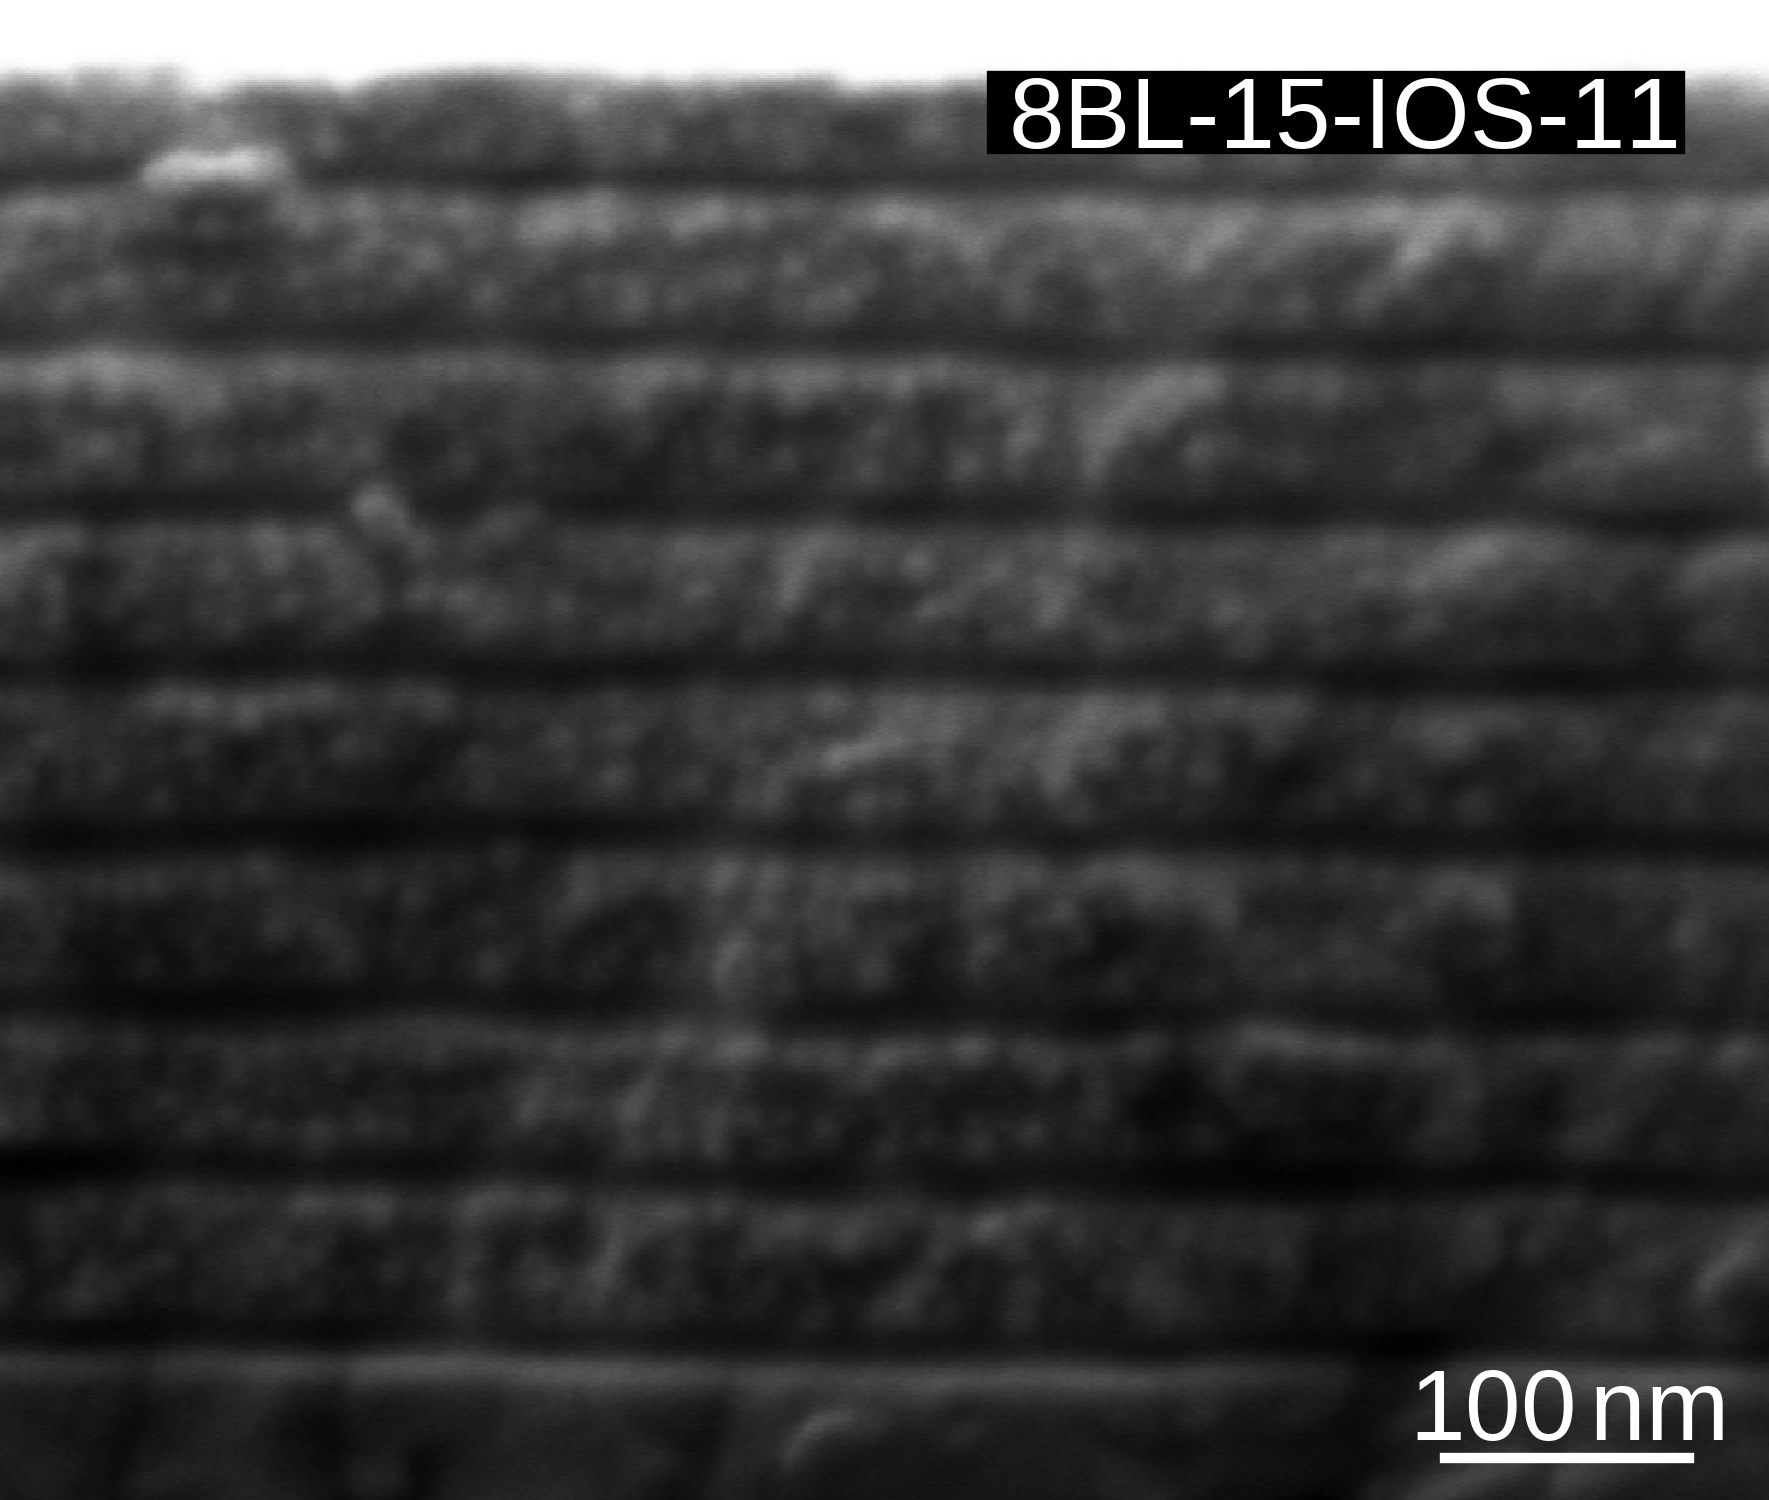
\includegraphics{looselyPackedNP_SEM_8BL-15-IOS-11}
    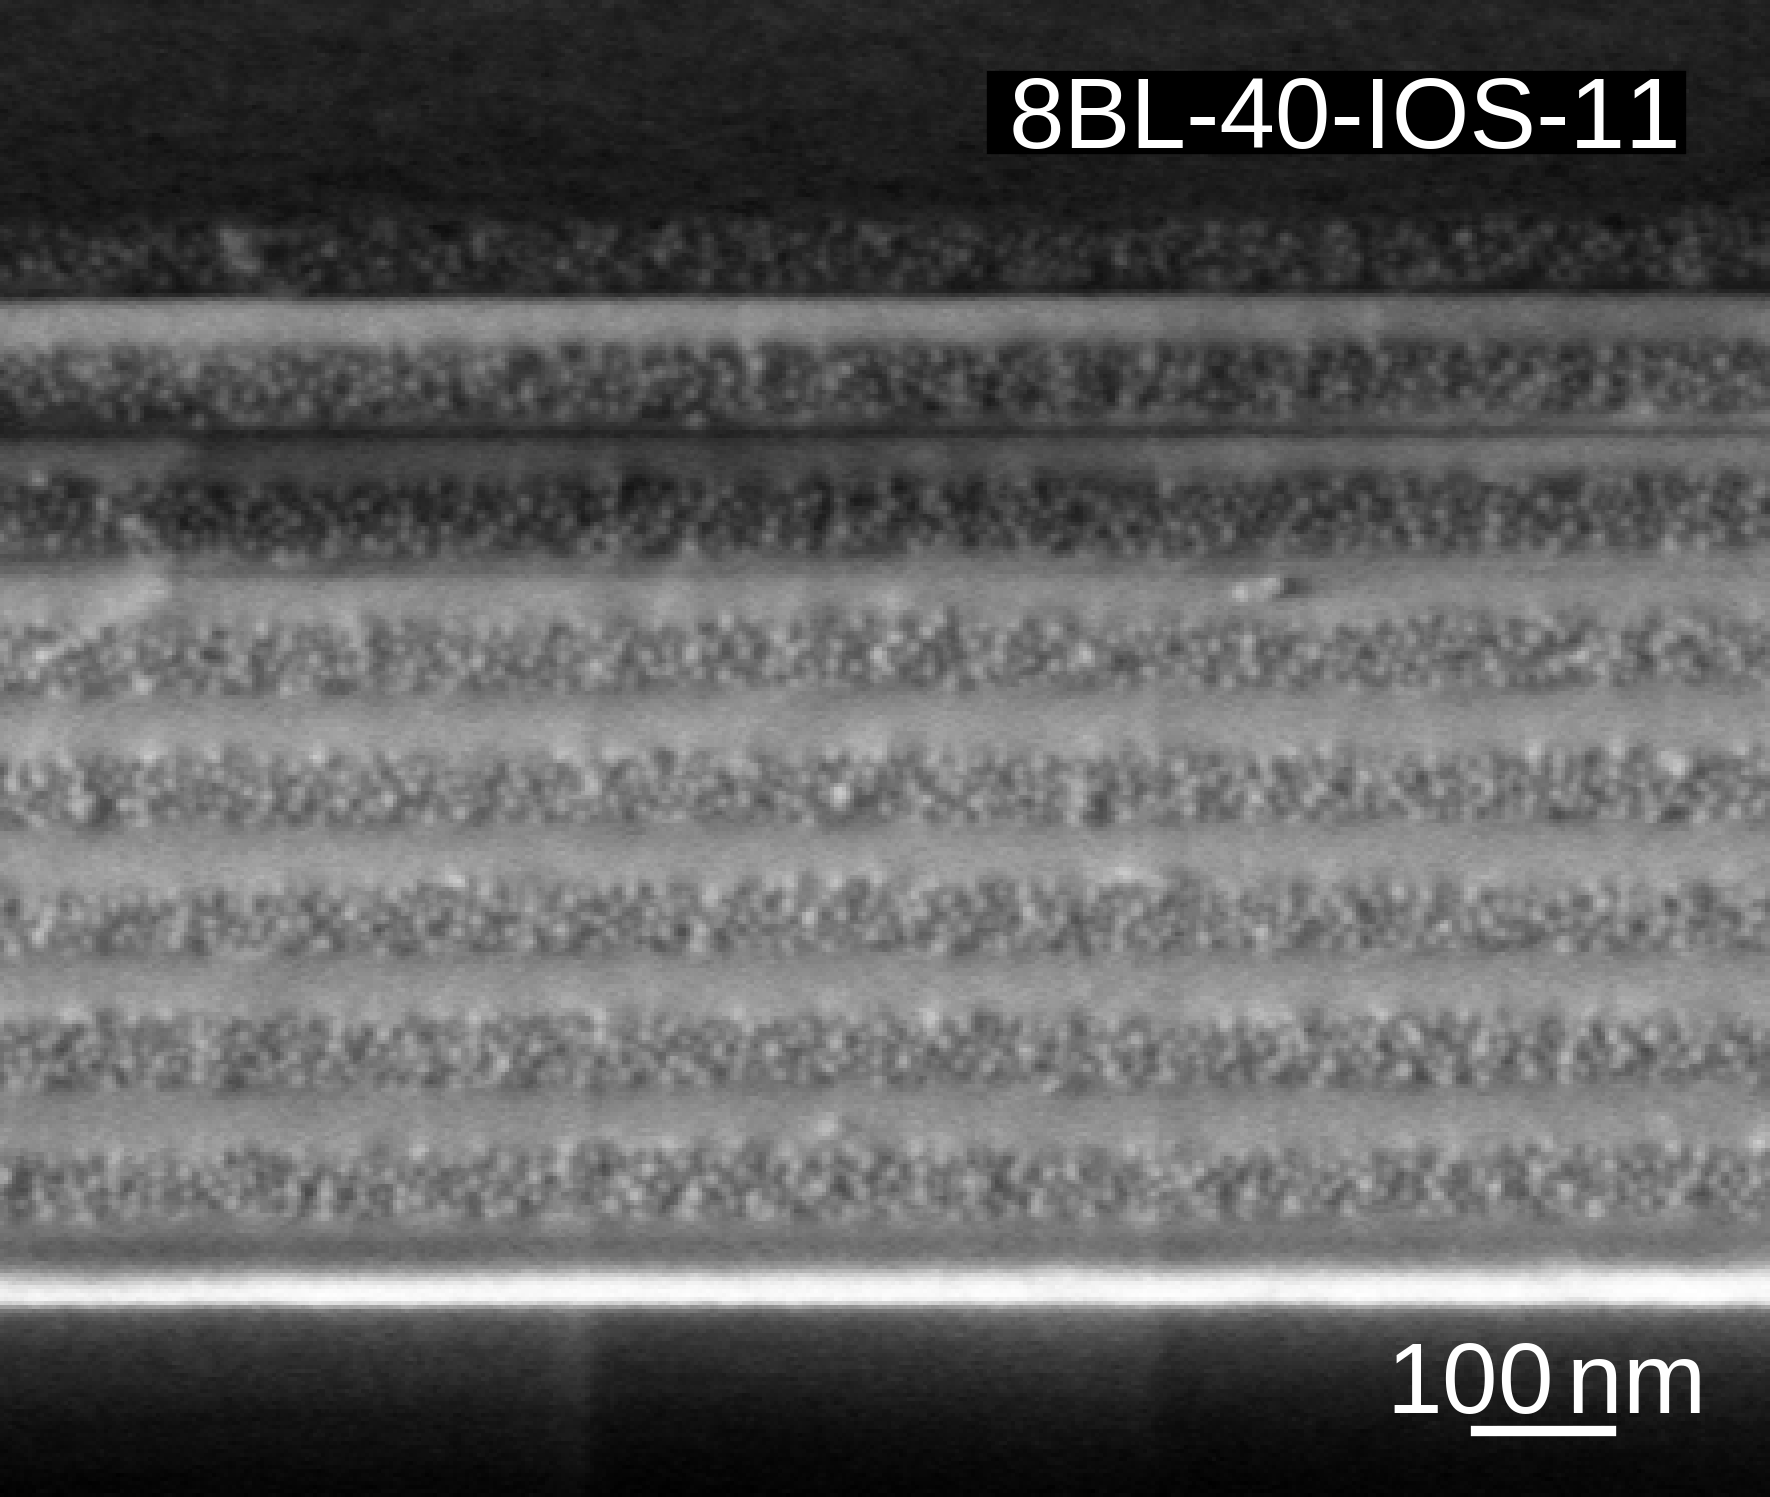
\includegraphics{looselyPackedNP_SEM_8BL-40-IOS-11}
    \caption{\label{fig:looselyPackedNP:bilayerStacks:sem11}SEM micrographs of the cross-section of 8BL-15-IOS-11 (left) and 8BL-40-IOS-11 (right).}
  \end{figure}
  \begin{figure}[tb]
    \centering
    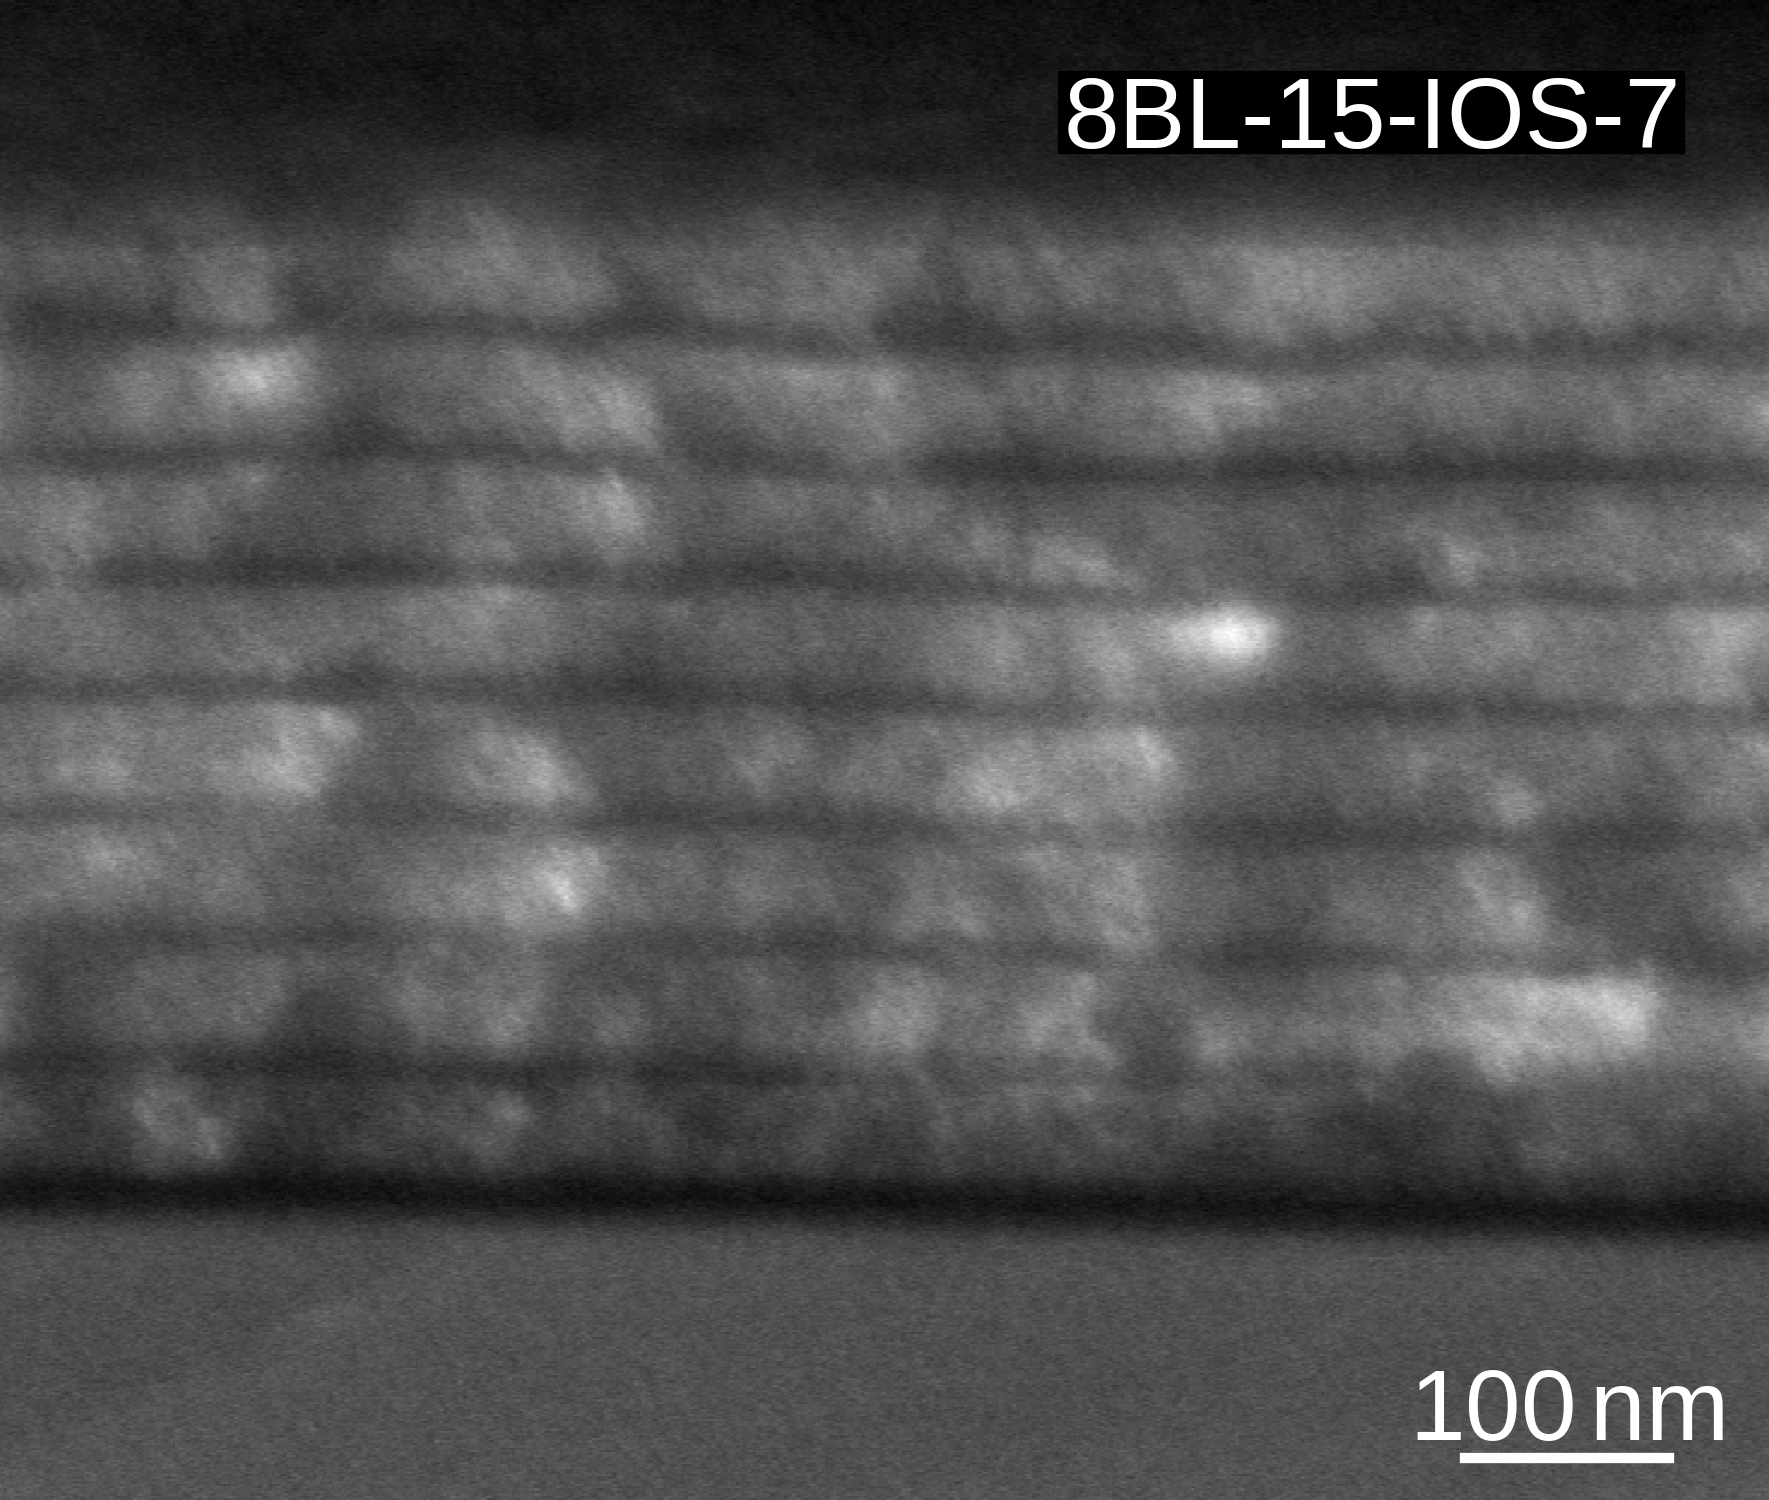
\includegraphics{looselyPackedNP_SEM_8BL-15-IOS-7}
    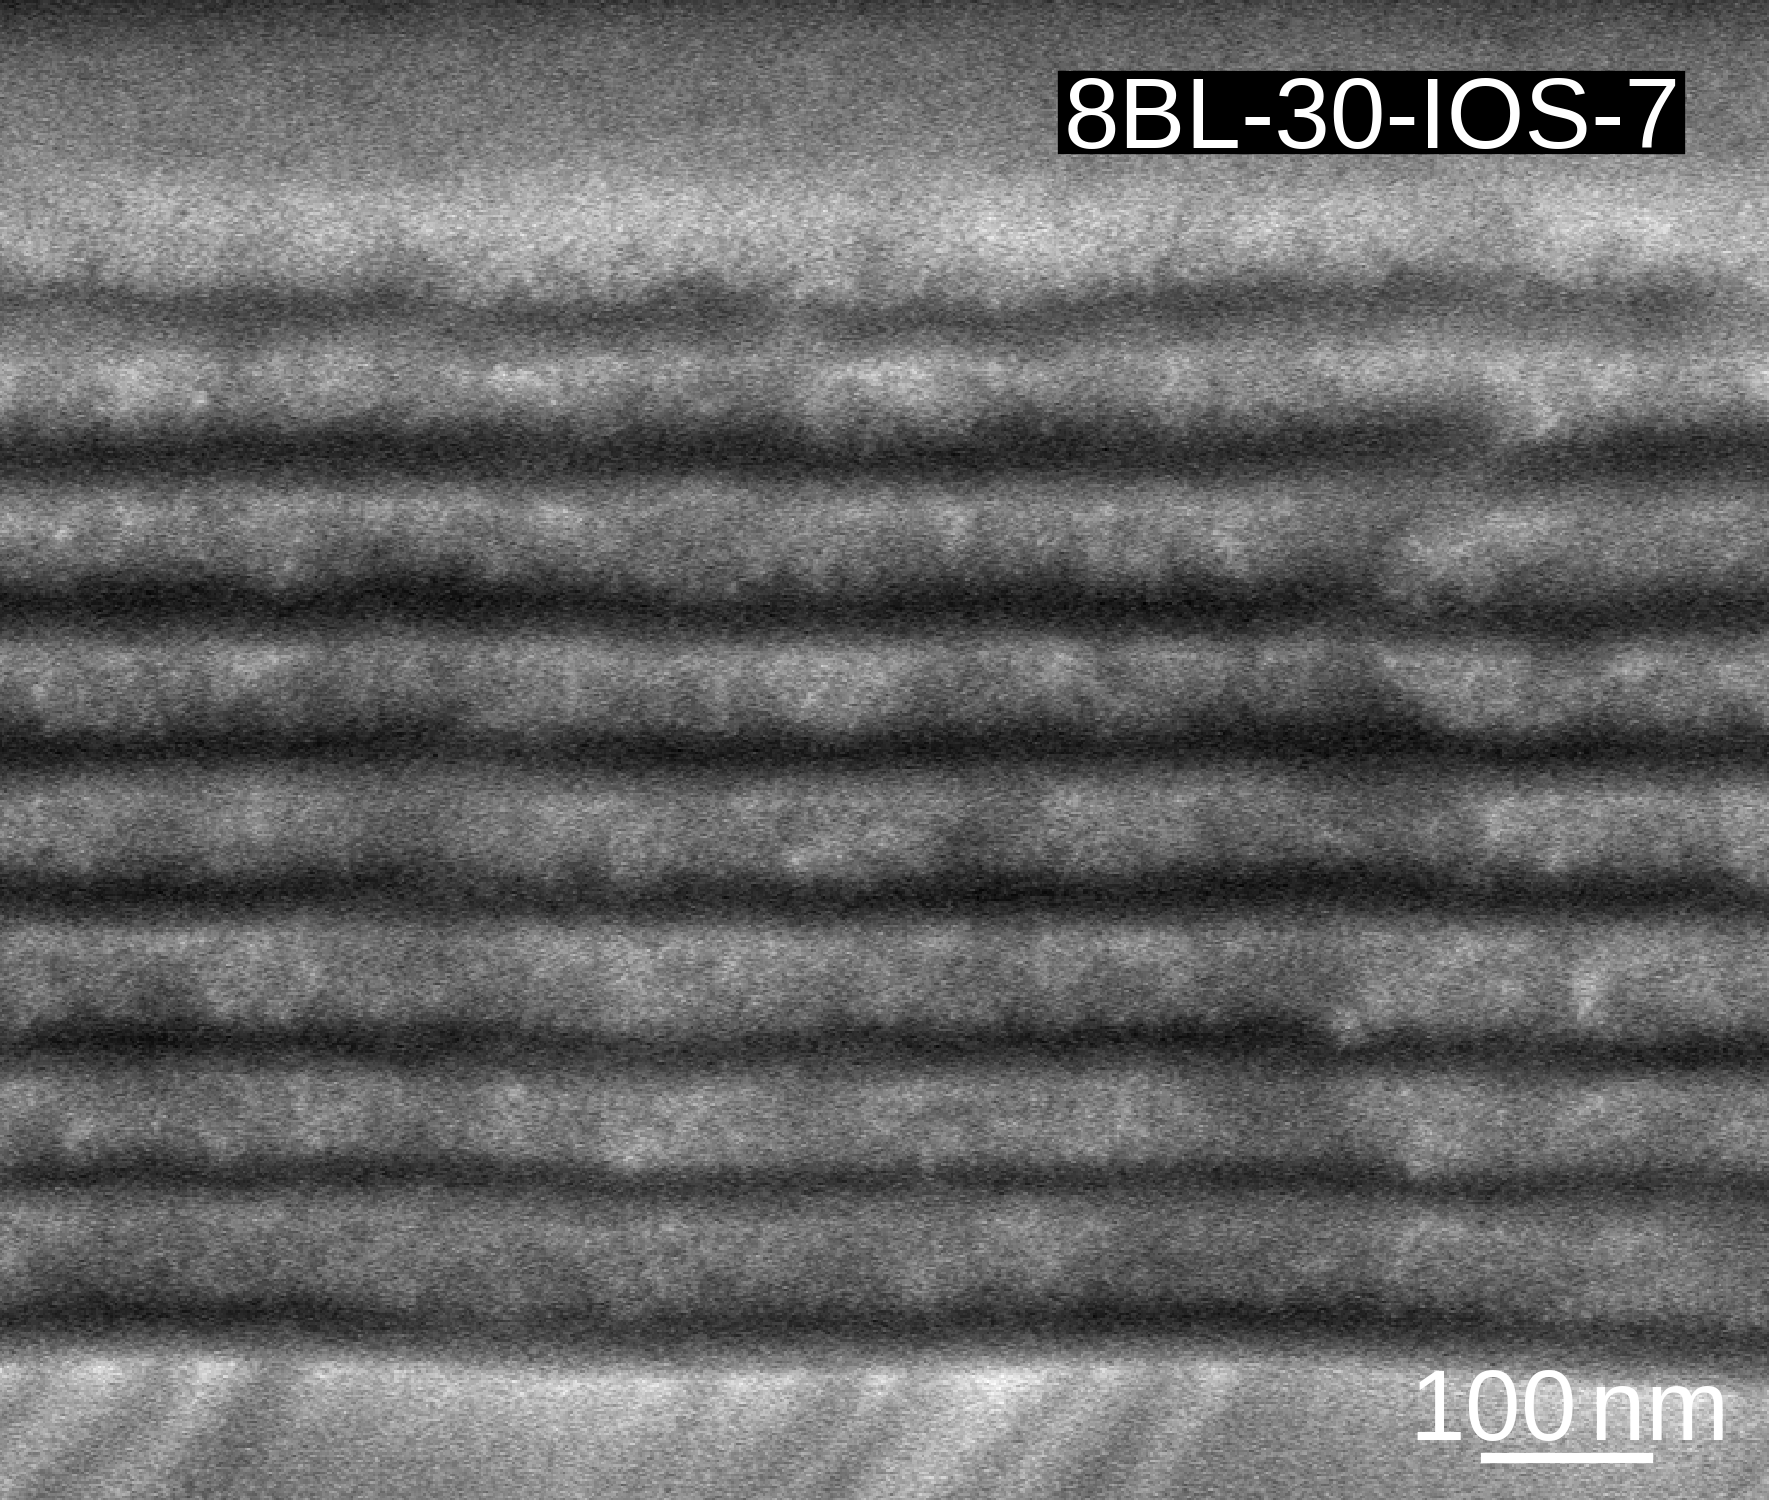
\includegraphics{looselyPackedNP_SEM_8BL-30-IOS-7}
    \caption{\label{fig:looselyPackedNP:bilayerStacks:sem7}Cross-sectional micrographs of 8BL-15-IOS-7 (left) and 8BL-30-IOS-7 (right).}
  \end{figure}

  The scanning electron microscopy images of the eight stacks of PMMA and IOS-11 nanospheres bilayers, shown in \reffig{fig:looselyPackedNP:bilayerStacks:sem11}, reveal the high quality and smooth layer structure of the provided samples.
  It is visible that the samples start with a PMMA layer and terminate with a nanoparticle layer, and the micrographs are used to estimate the mean layer thickness.
  For the bilayer stack samples from IOS-7 the SEM micrographs shown in \reffig{fig:looselyPackedNP:bilayerStacks:sem7} are used to evaluate the average layer thickness.
  The resulting mean value and standard deviation are tabulated in \reftab{tab:looselyPackedNP:bilayerStacks:semLayerThickness}.

  The variation of the the layer thickness is in the order of $3 - 5 \unit{nm}$ visible by the standard deviation.
  For the 8BL-x-IOS-11 samples, the nanoparticle layer thickness are in a comparable order of magnitude, with both being aproximately $50 \unit{nm}$ thick.
  For the samples from IOS-7, additionally to the intended PMMA thickness layer variation, a variation in the nanoparticle layer thickness is visible, being in the order of $40 \unit{nm}$ for 8-BL-15-IOS-7 and $60 \unit{nm}$ for 8BL-30-IOS-7.

  \begin{table}[!htbp]
    \centering
    \caption{\label{tab:looselyPackedNP:bilayerStacks:semLayerThickness}Mean layer thickness of the PMMA layers $d_\mathrm{PMMA}$ and the nanoparticle layers $d_\mathrm{NP}$ determined from the SEM micrographs.}
    \begin{tabular}{ c | l | l}
      \rule{0pt}{2ex} \textbf{SEM}  & $d_\mathrm{PMMA} \, / \unit{nm}$ & $d_\mathrm{NP} \, / \unit{nm}$ \\
      \hline
      8BL-15-IOS-11 & $13(2)$ & $50(5)$\\
      8BL-40-IOS-11 & $40(3)$ & $53(3)$\\
      8BL-15-IOS-7  & $13(2)$ & $37(3)$\\
      8BL-30-IOS-7  & $29(4)$ & $60(3)$\\
      \hline
    \end{tabular}
  \end{table}

\end{document}